\chapter{Crayon}
\label{cha:crayon}

In this section Crayon, a Python toolkit for benchmarking ML forecasting models, is introduced. Crayon contains a set of tools for making fair, accurate and reproducible comparisons between forecasting models. Crayon is open sourced and available on GitHub under the MIT license \cite{crayon_github}.

Crayon is based on the benchmarking architecture presented in chapter \ref{cha:designing}. Technically reproducible results are made through the use of three core technologies; Runtool configuration files for defining reproducible training jobs, Docker images containing the algorithm to benchmark and the public datasets available through Gluon-TS. In order to make benchmarks statistically reproducible, error metrics generated from benchmarks can be automatically compared through the Kolmogorov-Smirnov 2 sample hypothesis test. Crayon is error metric agnostic, meaning that any error metrics required for a certain domain can be used, thus enabling accurate comparisons between models. Additionally, the RMSE4D aggregation method presented in Chapter \ref{cha:designing} is used to rank distributions of error metrics.

Since it is common that machine learning workloads are executed in the cloud, as well as locally, both options are supported by Crayon. Since the runtool only supports executing training jobs in AWS SageMaker a custom backend is implemented for local execution.

\section{Architecture}

This section introduces the overall architecture of Crayon and important modules and concepts are briefly explained.
Crayon has three basic buliding blocks, \textit{Algorithm objects} \textit{Dataset objects} and \textit{Runtool configuration files} (configs). Algorithm objects and Dataset objects is an abstraction simplifying the writing of runtool config file for users and are used internally to generate one or more runtool configuration files. These generated configuration files have a single purpose, to enable technically reproducible benchmarks. In Figure \ref{fig:crayon_architecture} an overview of the five most important modules of Crayon is shown; Benchmarking, Verification, Scoring and the Tuning module. Furthermore, the central use of the BRF described in Chapter \ref{cha:designing} is shown.

The Benchmarking functionality showed on top in Figure \ref{fig:crayon_architecture} takes the path to runtool configuration file and uses the algorithm specified within it to generate four new config files, one for each dataset the algorithm should be benchmarked on. 100 backtests are then executed using each config to generate distributions of error metrics. These backtests can then be executed locally in a sequential manner or in parallel on AWS SageMaker. The recorded error distributions are then stored together with the config file to a BRF to enable statistical and technical reproducibility of the benchmark. After the benchmark is finished, the scoring functionality in Crayon is used to score the distribution of error metrics using the RMSE4D of the error distributions. This score is then ranked against the RMSE4D score of any other benchmarks stored in the BRF which used the same error metric.

Verifying benchmark performance leverages the statistical and technical reproducibility of the benchmarks in the BRF. Since the config used for previous benchmarks is stored in the BRF, a third party can repeat a benchmark as long as the docker image used and the BRF is available. After a benchmark is repeated, the verify module in Crayon can be used to assert statistical reproducibility through applying the kolmogorov smirnov 2 sample test on the two benchmarks error distributions. If the test passed, statistical reproducibility is achieved.

Since optimally tuned models are required for fair comparison as per the discussion in Chapter \ref{cha:designing}, grid search with repeated runs is implemented in Crayon. Grid search utilizes Algorithm and Dataset objects and a grid of hyperparameters to test. Provided these assets, the grid search generates one runtool config for each hyperparameter configuration and backtests it multiple times before aggregating the runs and evaluating the performance. After tuning finishes, the path to the best config is presented to the user.

This section introduced the high level workings of Crayon, the remainder of this chapter dives further into the features of Crayon with practical examples of various methods and tools.

\begin{figure}[htb]
  \centering
  \minipage{1.0\textwidth}
  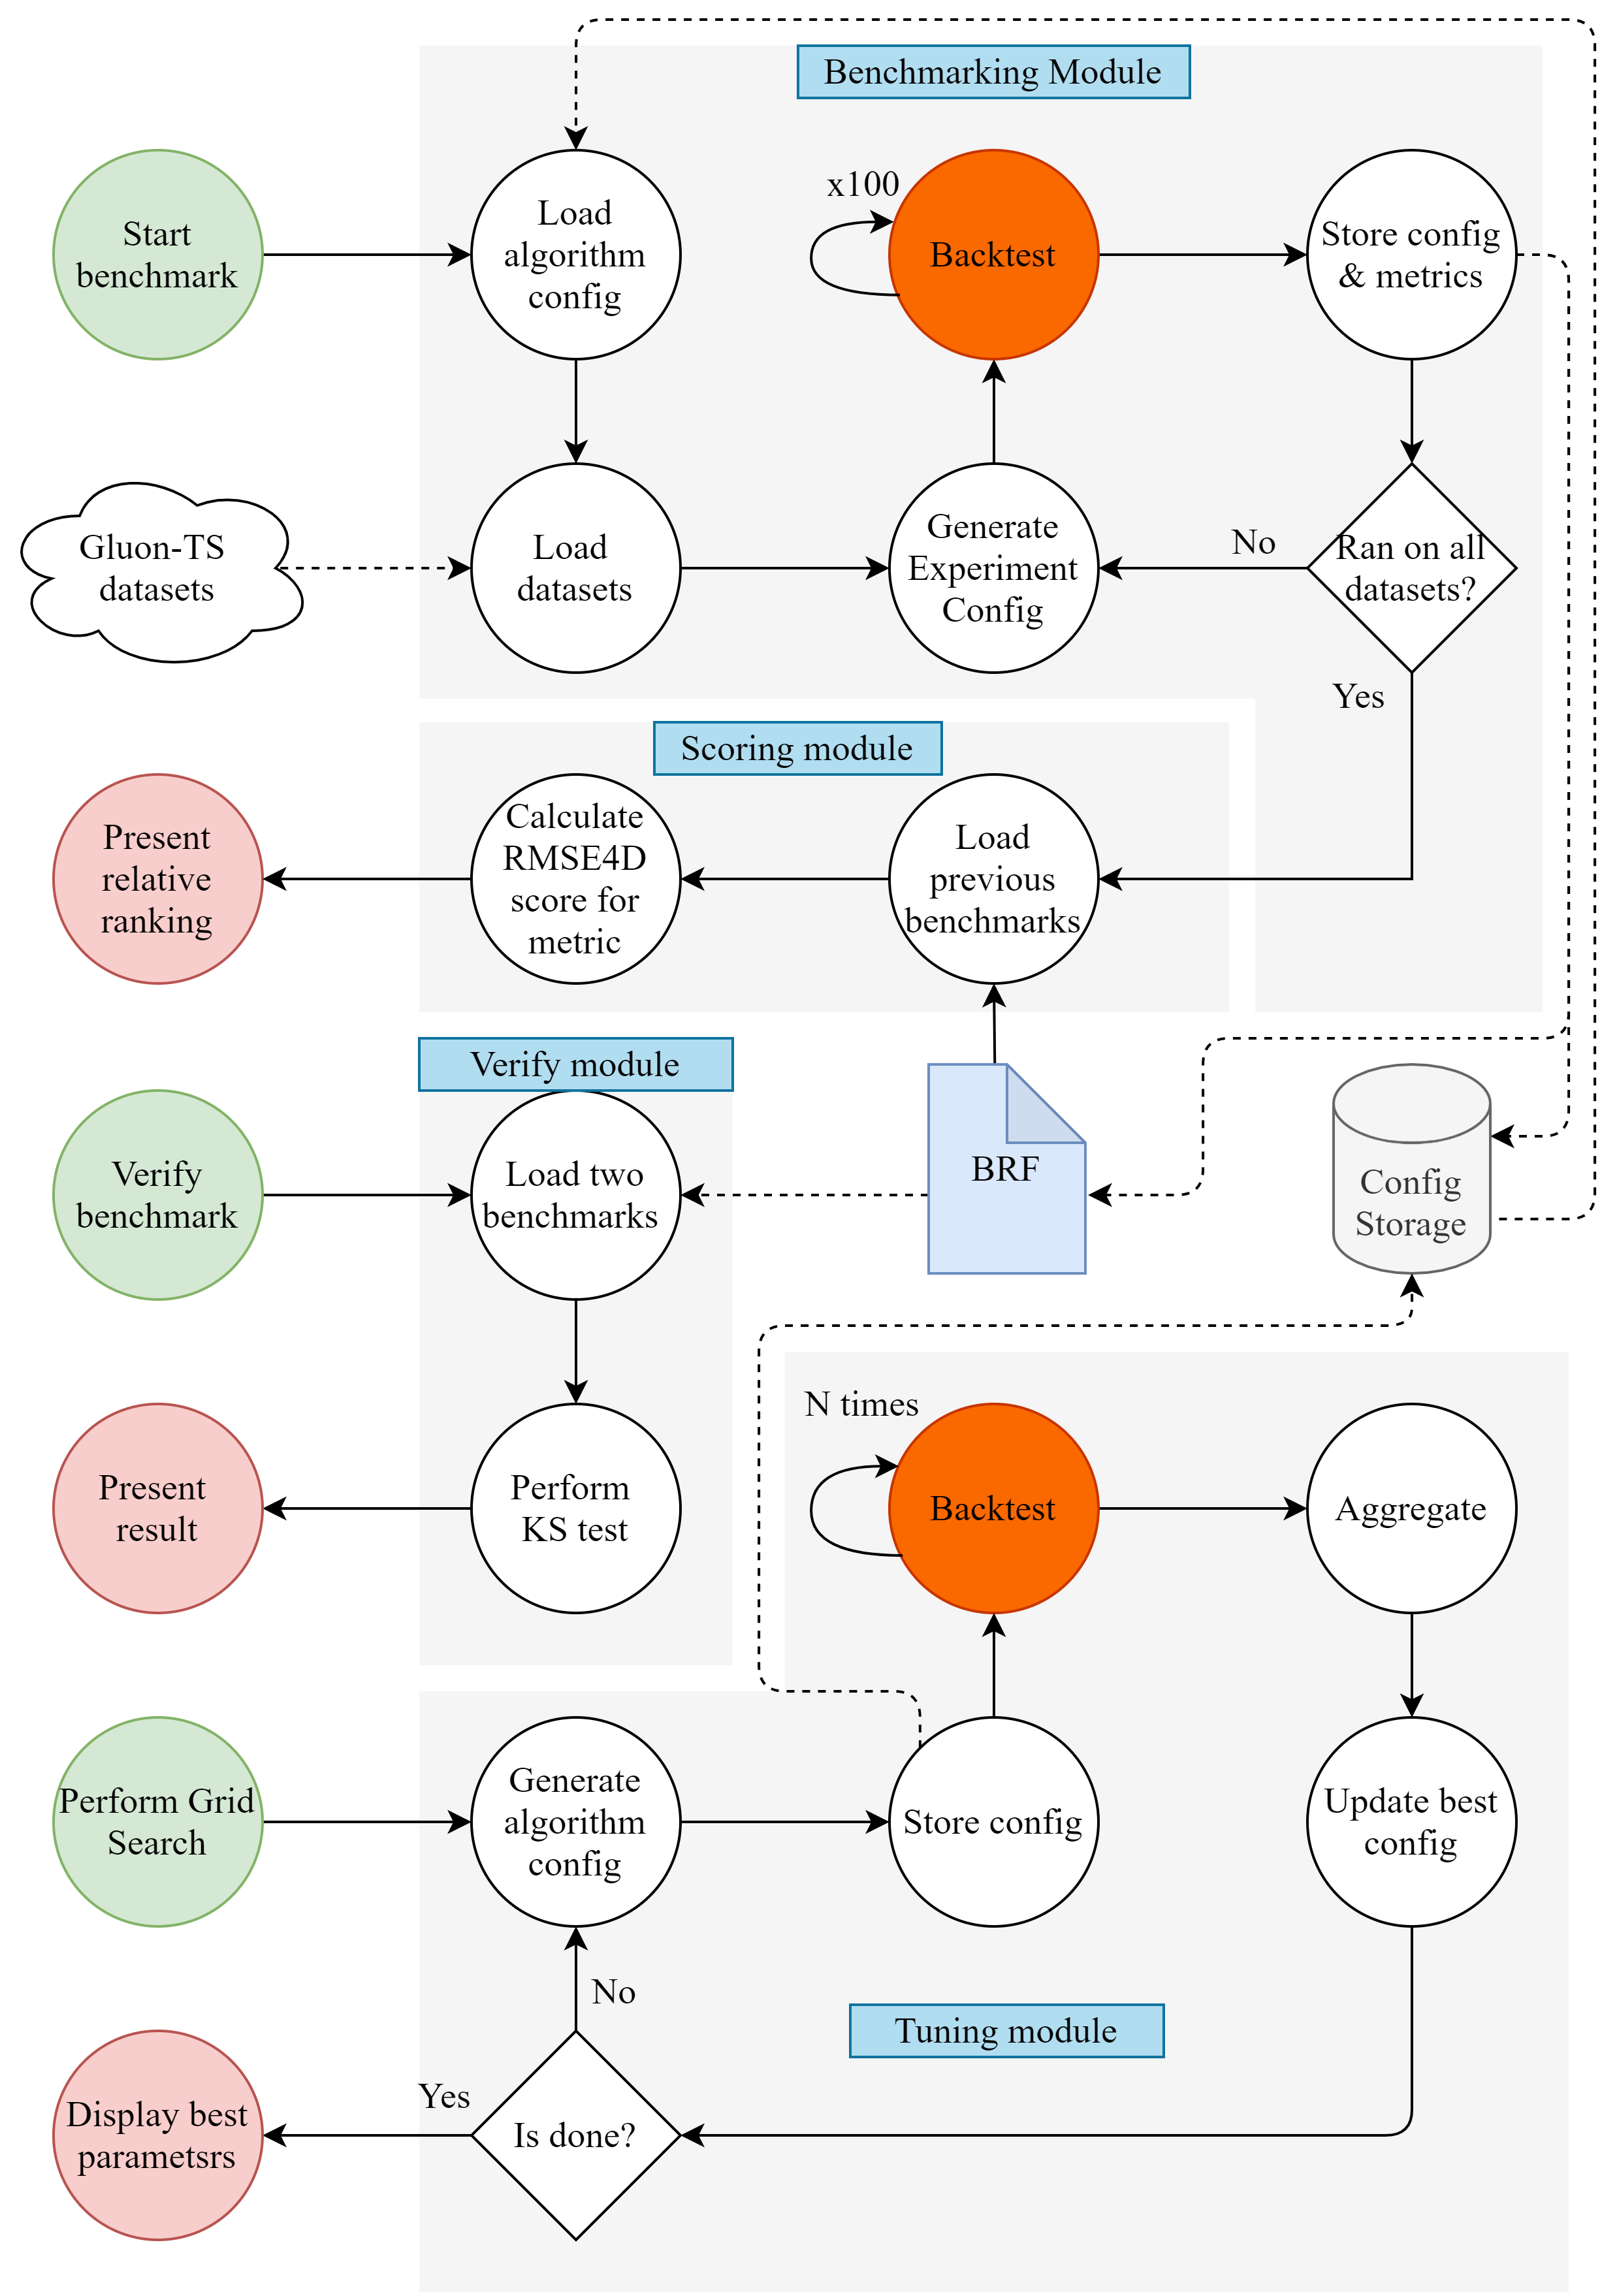
\includegraphics[width=\linewidth]{./img/crayon_architecture.png}
  \caption{Overview of the functionality in Crayon, start states are marked in green and end states in red, orange states can be executed locally or in the cloud.}
  \label{fig:crayon_architecture}
  \endminipage\hfill
\end{figure}
\clearpage

\section{Algorithms}
\label{crayon:algorithms}
In crayon, the \textit{Algorithms} class contains all the information needed in order to execute an algorithm contained in a Docker image stored either on AWS ECR or on the local machine. \textit{Algorithm} objects are the basic building blocks for performing hyperparameter tuning and for creating runtool configuration files.

An \textit{Algorithm} object contains information about the \textit{image} to run, the \textit{hyperparameters} to use. If the algorithm should be executed on SageMaker, the specific instance it should be run on can also be set using the \textit{instance} parameter. The \textit{Algorithm} class also optionally accepts a dictionary of regexes to the \textit{metrics} parameter. These regexes are used by SageMaker to extract metrics from an algorithms output. Default regexes for Gluon-TS algorithms are available in the \textit{crayon.utils} module. This parameter is not required when executing locally. In Listing \ref{code:algorithm} an example is shown of how the \textit{Algorithm} class is used.

\begin{figure}[h]
  \begin{lstlisting}[language=Python,label={code:algorithm},caption={Example of the Algorithm class.}]
from crayon import Algorithm
Algorithm(
  name="myalgo", 
  image="my_image", 
  instance="local",
  hyperparameters={...},
  metrics={"abs_error": ... }
)
  \end{lstlisting}
  % \caption{Example of the Algorithm class.}
  % \label{code:algorithm}

\end{figure}
\section{Datasets}
\label{crayon:datasets}
The Crayon \textit{Dataset} class wraps all the data needed to locate a dataset on your local machine or on AWS S3. It only takes two required parameters; the \textit{name} of the dataset \& the \textit{path} to the dataset on locally or on AWS S3.

The \textit{path} is a dict which points to the file location(s) of the dataset. If one has a train, test and validation dataset, the items in the \textit{path} will point to these versions of the dataset. Any \textit{meta} information one wish to provide about the dataset in question can be passed through the \textit{meta} parameter. In \ref{code:dataset} an example of how to use the Dataset class is presented.
\begin{figure}[h]
  \begin{lstlisting}[language=Python, label={code:dataset}, caption={Example of the Dataset class.}]
from crayon import Dataset
Dataset(
  name="electricity",
  path={
    "train": "file:///datasets/electricity/train/data.json",
    "test": "file:///datasets/electricity/test/data.json",
  },
  meta={...}
)
  \end{lstlisting}
\end{figure}
\section{Config Generation}
\label{'subsub:config_generation'}
This section discusses the different tools available in Crayon in order to create runtool compatible config files. These config files are a core part of the Crayon functionality and is used in several internal systems. Thus it is important to understand how these are generated and look like. For further information about how the config files function and additional functionality of them, see the section about the runtool (\ref{subsec:runtool}).

Through providing a \textit{Algorithm} object \& a \textit{Dataset} object to the \textit{generate\_config} function in Crayon, a configuration file compatible with the runtool is generated. The intention of this file is that by providing the config, the image used and the dataset to another person, that person could rerun your experiments with the exact same configuration. Internally Crayon uses the \textit{generate\_config} function in order to create tuning and benchmarking training jobs. See \ref{code:config_generation} for an example.
\begin{figure}
  \begin{lstlisting}[language=Python, label={code:config_generation}, caption={Config generation using Crayon}]
from crayon import Algorithm, Dataset, generate_config

# generate runtool configuration file
config = generate_config(
  Algorithm(
    name="myalgo",
    image="my_image",
    hyperparameters={"epochs": 10},
  ),
  Dataset(
    name="my_ds",
    path={
      "train": "/datasets/electricity/train/data.json",
      "test": "/datasets/electricity/test/data.json",
    },
  ),
  "/Users/freccero/Documents/config.yml",
)
\end{lstlisting}
\end{figure}

After executing the code in \ref{code:config_generation}, a config file is stored to the path provided to \textit{generate\_config}, in this case the config file is stored to \textit{/Users/freccero/Documents/config.yml}. The config file generated by the code in \ref{code:config_generation} is displayed in Listing \ref{code:generated_config}.
\begin{figure}
  \begin{lstlisting}[label={code:generated_config}, caption={Generated configurations file.}]
my_ds:
  meta: {}
  name: my_ds
  path:
    test: file:///datasets/electricity/test/data.json
    train: file://datasets/electricity/train/data.json
myalgo:
  hyperparameters:
    epochs: 10
  image: my_image
  instance: local
  name: myalgo
\end{lstlisting}
\end{figure}


If one does not have a custom dataset but instead wishes to use a reference dataset for training and evaluating the algorithm on, it is possible to use the datasets in Gluon-TS. The \textit{get\_gluonts\_datasets} function downloads any number of Gluon-TS datasets onto the local machine and generates a list of Datasets objects which can be passed to the  \textit{generate\_config} function. Example code for doing so is shown in \ref{code:config_generation_gluonts} with the output of the code displayed in \ref{output:config_generation_gluonts}.

\begin{figure}[h]
  \begin{lstlisting}[language=Python, label={code:config_generation_gluonts}, caption={Config generation using Crayon with gluonts datasets}]
from crayon import Algorithm, Dataset, generate_config, get_gluonts_datasets
import yaml

# generate runtool configuration file
config = generate_config(
  Algorithm(
    name="myalgo",
    image="my_image",
    hyperparameters={"epochs": 10},
  ),
  get_gluonts_datasets(["electricity"]),
  "/Users/freccero/Documents/config.yml",
)

print(yaml.dump(config))
    \end{lstlisting}
\end{figure}
\begin{figure}
  \begin{lstlisting}[label={output:config_generation_gluonts}, caption={Output when executing Code Fragment \ref{code:config_generation_gluonts}}]
electricity:
  meta:
    feat_dynamic_cat: []
    feat_dynamic_real: []
    feat_static_cat:
    - cardinality: '321'
      name: feat_static_cat
    feat_static_real: []
    freq: 1H
    prediction_length: 24
    target: null
  name: electricity
  path:
    test: file:///Users/freccero/.mxnet/gluon-ts/datasets/electricity/test/data.json
    train: file:///Users/freccero/.mxnet/gluon-ts/datasets/electricity/train/data.json
myalgo:
  hyperparameters:
    epochs: 10
  image: my_image
  instance: local
  metrics: null
  name: myalgo
    \end{lstlisting}
\end{figure}





\section{Training}
Given a valid runtool config file Crayon uses this file to start training jobs locally or on AWS SageMaker. The provided config file can be either written by hand or generated using Crayon as described in \ref{'subsub:config_generation'}.

A training job is started by calling the \textit{crayon.run\_config} method with the config. The experiment to run is defined using the mathematical operators + and * as described in Section \ref{subsec:runtool}.

The \textit{crayon.run\_config} function returns a \textit{Jobs} object which makes it easy to investigate training results as it stores all metrics reported by the algorithms across all started jobs to a pandas DataFrame.

\subsection{Local Training}
If a config is to be run locally, algorithm defined in the config need to point to an image which is available on the users machine. The image used should be valid for use with AWS SageMaker. Furthermore, any datasets which the algorithm should be trained on should also be available on the local machine. For details of what constitutes a valid SageMaker image, refer to the documentation of SageMaker \cite{sagemaker_docker_documentation}.

In listing \ref{config:local_training} an example configuration file for local training is displayed and in \ref{code:local_training} code for training the algorithm on the dataset in the config is presented.
\begin{figure}[h]
  \begin{lstlisting}[label={config:local_training}, caption={Config file for running local training jobs}]
my_algo:
  image: gluonts:cpu_new
  hyperparameters:
    freq: H
    prediction_length: 24
    forecaster_name: gluonts.model.deepar.DeepAREstimator
  instance: local

my_dataset:
  path:
    train: file:///datasets/electricity/train/data.json
    test: file:///datasets/electricity/test/data.json
  \end{lstlisting}
\end{figure}
\begin{figure}[h]
  \begin{lstlisting}[language=Python, label={code:local_training}, caption={Code for running local training jobs using Crayon}]
from crayon import run_config

jobs = run_config(
  config="config.yml",
  combination="config.my_algo * config.my_dataset",
)
  \end{lstlisting}
\end{figure}


By executing the code in Code Fragment \ref{code:local_training} Crayon will use the runtool to load the config in \ref{config:local_training} and start training jobs locally through the \textit{local\_run} method of the runtool. The jobs will be executed sequentially. After the jobs finish, Crayon looks for a file named \textit{agg\_metrics.json} or \textit{metrics.json} in the output directory for each job. This file is expected to contain any metrics reported by the algorithm being trained. An example json file is shown in \ref{output:local_job_output} for reference.

\begin{figure}
  \begin{lstlisting}[label={output:local_job_output}, caption=Example of a training job output file such as \textit{metrics.json} or \textit{agg\_metrics.json}]
{
  "MSE": 6703174.123610994,
  "abs_error": 37402126.36717987,
  "MASE": 1.62229213532052,
  "MAPE": 0.23736356524438723
}
\end{lstlisting}
\end{figure}


\subsection{Cloud Training}
\label{sec:cloud_training}
Executing training jobs in SageMaker is done similarly as when starting them locally, but with some alterations to the config file and to the python script.

The config file needs to refer to an image available in ECR of the AWS account that is to be used. Further, the \textit{instance} in the config file must match one of the instance types which SageMaker offers. Any metrics which the algorithm outputs during training such as accuracy metrics or similar must have a corresponding regex under the metrics tag in the config file. This regex is used by SageMaker to parse the algorithm output for metrics. The final change to the config which needs to be done for running on SageMaker is that any datasets needs to be stored in an AWS S3 bucket instead of locally.

In addition to the above changes to the config file, three further parameters are required by the \textit{run\_config} function in the Python script.

\begin{enumerate}
  \item \textit{role\_arn} - The AWS IAM Role  which authorizes Crayon to start training jobs on SageMaker.
  \item \textit{bucket} - The AWS S3 bucket where any artifacts of the training job should be stored.
  \item \textit{session} - A \textit{boto3.Session} object which Crayon will use to interact with SageMaker.
\end{enumerate}

The IAM Role requires permissions to start training jobs on sagemaker, pull AWS ECR images, and read/write access to the provided S3 bucket. For information about how to create a IAM Role with the proper permissions as well as an S3 bucket please refer to the AWS documentation for these two services \cite{iam_website,s3_website}.

In Listing \ref{config:cloud_training}, an example configuration file is displayed which can be used to train on AWS SageMaker and in \ref{code:cloud_training} an example python file is presented which given a config dispatches training jobs to SageMaker using the \textit{run\_config} function of Crayon.

\begin{figure}[h]
  \begin{lstlisting}[label={config:cloud_training}, caption={Config file for running training jobs on SageMaker.}]
my_algo:
  image: 012345678901.dkr.ecr.eu-west-1.amazonaws.com/gluonts:2020-11-01
  hyperparameters:
  freq: H
  prediction_length: 24
  forecaster_name: gluonts.model.deepar.DeepAREstimator 
  instance: ml.m5.xlarge 
  metrics:
  abs_error: 'abs_error\): (\d+\.\d+)'

my_dataset:
  path:
  train: s3://gluonts-run-tool/gluon_ts_datasets/constant/train/data.json
  test: s3://gluonts-run-tool/gluon_ts_datasets/constant/test/data.json
      
  \end{lstlisting}
  % \end{figure}
  % \begin{figure}[h]
  \begin{lstlisting}[language=Python, label={code:cloud_training}, caption={Code for running training jobs on AWS SageMaker using Crayon}]
from crayon import run_config
import boto3

jobs = run_config(
  config="config.yml",
  combination="config.my_algo * config.my_dataset",
  role_arn="arn:aws:iam::012345678901:role/service-role/my_role",
  bucket="my_bucket",
  session=boto3.Session(),
)
    \end{lstlisting}

\end{figure}

\section{Tuning}
In order to use Crayon as a benchmarking tool, it is advised that each algorithm has been suitably tuned to the datasets which it should run on. This is required since comparing a finely tuned model with an undertuned model will result in unfair comparisons being made.

Grid search is a common strategy used when tuning algorithm. When tuning using grid search, one creates for each hyperparameter a list of values which that hyperparameter can take. Thereafter the algorithm is then run for each combination of these parameters. The hyperparameter combination resulting in the best results is then returned as the optimal hyperparameter combination to use.

Below I present how an algorithm can be tuned using the grid-search functionality in Crayon.

\subsection{Grid-Search}
Grid search is done using the \textit{grid\_search} function in the \textit{Crayon.Tuner} module. The \textit{grid\_search} function is implemented based on the architecture suggested in \ref{sec:hpo} with some additional features. Since multiple runs of an algorithm generates a small distribution of values, the method used for aggregating these is customizable, per default the mean is taken. Further, since different metrics may optimize towards different values, a custom method for comparing values can be passed, per default lower aggregate errors are better. Each hyperparameter configuration generated by \textit{grid\_search} is stored into a runtool configuration file. This simplifes the benchmarking of a tuned algorithm as the generated runtool config file can be used directly by the \textit{crayon.benchmark} method presented in Section \ref{subsec:benchmarking}.

An overview of the features of the \textit{grid\_search} module is displayed in Figure \ref{features_grid_search}:

\begin{figure}[h]
  \begin{itemize}
    \item Performs grid search with both static and changing parameters.
    \item Each hyperparameter combination can be rerun multiple times to handle non-deterministic algorithms
    \item Allows passing a custom function for aggregating error metrics from jobs.
    \item Allows passing of a custom scoring function for evaluating jobs.
    \item Generates runtool configuration files for each combination of hyperparameters.
  \end{itemize}
  \caption{Features of the grid search functionality in Crayon.}
  \label{features_grid_search}
\end{figure}


\subsubsection{Overview of the grid\_search function in Crayon}
\begin{figure}
  \begin{lstlisting}[language=Python, label={code:grid_search_signature}, caption={Parameters of the grid search functionality in Crayon.}]
def grid_search(
  changing_hyperparameters: dict,
  target_metric: str,
  dataset: Dataset,
  algorithm: Algorithm,
  output_dir: str = crayon_dir().resolve(),
  aggregation_function: Callable = statistics.mean,
  evaluation_function: Callable = lambda new, old: new < old,
  run_locally: bool = True,
  **kwargs,
) -> GridSearchResults:
    \end{lstlisting}
\end{figure}
In Code Fragment \ref{code:grid_search_signature} the signature for the \textit{grid\_search} method of Crayon is displayed. Each of the parameters of this method will here be presented and in Code Fragment \ref{code:grid_search_local} an example of how to perform grid search locally is presented.

In Code Fragment \ref{code:grid_search_signature} \textit{changing\_hyperparameters} are the hyperparameters which are to be tuned. This parameter takes a dictionary where the keys are the hyperparameters to tune and the value is a list of values which they should take. The \textit{target\_metric} parameter selects which metric that the algorithm outputs should be optimized for. Further, the grid search takes a \textit{crayon.Dataset} and a \textit{crayon.Algorithm} (see Sections \ref{crayon:algorithms} \& \ref{crayon:datasets}). Any hyperparameters defined within the \textit{algorithm} stays the same for each run in the training loop. The \textit{output\_dir} determines where the Runtool configuration files created for each hyperparameter combination will be stored.

The \textit{aggregation\_function} is used to merge the results if each configuration should be run more than once. Per default this is done is by taking the mean of the recorded values. Through passing a custom function to the \textit{aggregation\_function} parameter one can override this behaviour. This function needs to take a list of numbers as a parameters and it needs to return a single value. In Code Fragment \ref{code:grid_search_local} the \textit{mean} function is provided from the \textit{statistics} module in the standard library of Python.

The \textit{evaluation\_function} is used to determine whether the results of the most recent hyperparameter combination were better than the best seen hyperparameter combination so far. The default behaviour defines that if the new value of the target metric is lower than the best so far, it is better. This makes sense whenever one wishes to minimize the target metric, i.e., an absolute error of 10 is better then an absolute error of 100. However, for other target metrics, different behaviour may be more suitable. Providing a function which takes two parameters, the new value and the old value and compares these to the \textit{evaluation\_function} parameter the behaviour is customized. The \textit{run\_locally} parameter determines if the jobs should be executed on the local machine or on AWS SageMaker. Any additional parameters passed is forwarded to the \textit{crayon.run\_config} function for each training job. Thus, for executing in SageMaker the parameters defined in Section \ref{sec:cloud_training} need to be passed in addition.

In Code Fragment \ref{code:grid_search_local} grid search is performed on an image containing gluonts. The algorithm being tuned in Gluon-TS is the DeepAREstimator with the hyperparameters \textit{freq} and \textit{prediction\_length} being the same for each training job. The grid search tries to minimizing the average value of the \textit{abs\_error} metric over two runs for each hyperparameter combination. The hyperparameters that are tuned are the \textit{epochs} and the \textit{context\_length}.
\begin{figure}
  \begin{lstlisting}[language=Python, label={code:grid_search_local}, caption={Grid search running locally.}]
grid_search(
  algorithm=Algorithm(
    name="deepar",
    image="gluonts_cpu",
    hyperparameters={
      "freq": "D",
      "prediction_length": 7,
      "forecaster_name": "gluonts.model.deepar.DeepAREstimator",
    },
  ),
  dataset=Dataset(
    name="electricity",
    path={
      "train": "file:///electricity/train/data.json",
      "test": "file:///electricity/test/data.json",
    },
  ),
  runs=2,
  target_metric="abs_error",
  aggregation_function = statistics.mean, 
  evaluation_function = lambda new, old: new < old,
  changing_hyperparameters={
    "epochs": [1, 5],
    "context_length": [1, 5],
  }
)
  \end{lstlisting}
\end{figure}

% By setting the \textit{run\_locally} parameter to False we tell Crayon to execute the training on SageMaker instead of locally. In order to make this work, we need to provide the an AWS S3 bucket, an AWS IAM role and a boto3 Session object. See Section \ref{sec:cloud_training} for more information about these.
% An example of how grid search can be executed on SageMaker is presented in \ref{code:grid_search_cloud}.
% \begin{figure}
%   \begin{lstlisting}[language=Python, label={code:grid_search_cloud}, caption={Grid search running on SageMaker.}]
% from crayon import (
%     GLUONTS_METRICS, Algorithm, Dataset, grid_search
% )
% import boto3

% grid_search(
%   role_arn="arn:aws:iam::012345678901:role/my_role",
%   bucket="my_bucket",
%   run_locally=False,
%   session=boto3.Session(),
%   algorithm=Algorithm(
%     name="deepar",
%     image="my_ecr_url/gluonts/cpu",
%     hyperparameters={
%       "freq": "D",
%       "prediction_length": 7,
%       "forecaster_name": "gluonts.model.deepar.DeepAREstimator",
%     },
%     metrics=GLUONTS_METRICS,
%     instance="ml.m5.xlarge",
%   ),
%   dataset=Dataset(
%     name="electricity",
%     path={
%       "train": "s3://electricity/train/data.json",
%       "test": "s3://electricity/test/data.json",
%     },
%   ),
%   runs=2,
%   target_metric="abs_error",
%   aggregation_function = statistics.mean, 
%   evaluation_function = lambda new, old: new < old,
%   changing_hyperparameters={
%     "epochs": [1, 5],
%     "context_length": [1, 5],
%   }
% )
%     \end{lstlisting}
% \end{figure}
\section{Benchmarking}
\label{subsec:benchmarking}
One of the key components of Crayon is the benchmarking module. This module compares algorithms by backtesting them on four datasets with different characteristics; \textit{M5}, \textit{M4 Daily}, \textit{Electricity} and \textit{Solar Energy}. These datasets were chosen since they exhibit complimentary characteristics as per the discussion in \ref{sec:dataset_analysis}.

To benchmark an algorithm via Crayon a config file describing the algorithm needs to be passed. Furthermore, one must pass which target metric should be the target for the benchmark, i.e. absolute error, MASE, MAPE or any other metric reported by the benchmarked algorithm. Crayon then backtests the algorithm on each dataset 100 times in order to build up a distribution of the target metric. The value 100 was chosen as it is in the middle of the boundraries identified in Section \ref{sec:compairing_hypothesis_tests}. After the error metric distributions have been generated, RMSE4D described in Section \ref{sec:ranking_distributions} is used to compare the errors from the benchmark with previously run benchmarks. A lower value of RMSE4D is better.

As the benchmark is run on multiple datasets, it is important to provide tuned models for each. This is done by appending the dataset name to the algorithm name in the config file so that each algorithm defined in the config file has the structure: \(<algorithm\_name>\_<dataset\_name>\). In Code Fragment \ref{config:benchmarking} an example config file for benchmarking is presented. Note the two hyperparameter configurations of DeepAR in the config, this indicates that different hyperparameters is used for the electricity dataset.

\begin{figure}
  \begin{lstlisting}[language=Python, label={config:benchmarking}, caption={Config file for benchmarking with Crayon. Note that \textit{deepar\_electricity} has a different hyperparameter configuration thus these hyperparameters are used when benchmarking the algorithm on the electricity dataset. For all other datasets, the default algorithm definition \textit{deepar} is used.}]
deepar:
  name: deepar
  image: gluonts:cpu_new
  hyperparameters:
    epochs: 1
    freq:
      $eval: $trial.dataset.meta.freq
    prediction_length:
      $eval: 2 * $trial.dataset.meta.prediction_length
    context_length:
      $eval: 2 * $trial.algorithm.hyperparameters.prediction_length
    forecaster_name: gluonts.model.deepar.DeepAREstimator    
  instance: local

deepar_electricity:
  $from: deepar
  hyperparameters:
    epochs: 2
    \end{lstlisting}

  \begin{lstlisting}[language=Python, label={code:benchmarking}, caption={Python script for starting a benchmarking run using Crayon.}]
from crayon import benchmark

benchmark(
  algorithm_config="config.yml",
  algorithm_name="deepar",
  benchmark_id="my_benchmark",
  target_metric="MASE",
)
    \end{lstlisting}
\end{figure}

After the 100 backtests for each dataset has finished, the recorded error distributions are stored to a file on the local machine. This file also contains the \textit{id} of the benchmark, as well as the config used to create the training jobs. Also the \textit{Jobs} object which was generated from the benchmark are stored into this file. The Jobs objects contain the metrics recorded for a certain Job. The file where these values are stored was referred to as the Benchmark Result File (BRF) in Chapter \ref{cha:designing}. In future versions of Crayon, the BRF could be handled by some centralized storage server instead of locally, however this is out of the scope of the thesis.

\section{Verifying Benchmark Performance}
In \ref{sec:reproduce_benchmarks} an architecture for making benchmarks statistically reproducible was presented. In essence, statistical reproducibility of benchmarks can be made through applying a hypothesis test on the error metric distributions generated by the two benchmarks. Since, in Crayon, each benchmark consists of four distributions of error metrics, one for each dataset, four hypothesis tests need to be performed.

The \textit{Crayon.verify} function in Crayon is based on the architecture proposed in \ref{sec:reproduce_benchmarks}. \textit{Crayon.verify} takes the paths to two BRF files generated by benchmarks. Further, two Benchmark IDs are required in order to identify which benchmarks in the respective files should be verified against each other. The investigation in Section \ref{sec:compairing_hypothesis_tests} concluded that the Kolmogorov Smirnov 2 Sample Test (KS test) is suitable for comparing distributions of error metrics. This test is thus chosen for use in Crayon for verifying benchmarks. Since different metrics are supported by the benchmarking module, the specific metric distribution to verify is required by the \textit{verify} function.

In Code Fragment \ref{code:verify} an example of the \textit{crayon.verify} function is presented. There, two benchmarks from different BRFs are verified against each other using the KS test with respect to the MASE metric. Thus, the KS test is applied to the distributions of the MASE metric for each dataset in turn. If the KS test rejects the two distributions to be samples from the same underlying distribution the algorithms cannot be verified. In Code Fragment \ref{code:outputverification} example output after executing Code Fragment \ref{code:verify} is presented.

\begin{figure}
  \begin{lstlisting}[language=Python, label={code:verify}, caption={Verifying whether two benchmarks are performed by the same algorithm.}]
from crayon import verify

verify(
    id_1="my_benchmark",
    id_1_results_file="BRF_1.yml", 
    id_2="someone_elses_benchmark",
    id_2_results_file="BRF_2.yml",
    target_metric="MASE",
)
\end{lstlisting}
\end{figure}
\begin{figure}
  \begin{lstlisting}[language=bash, label={code:outputverification}, caption={Output from Code Fragment \ref{code:verify}}]
    Algorithm verified on dataset electricity
    Algorithm verified on dataset m4_daily
    Algorithm verified on dataset m5
    Algorithm verified on dataset solar_energy
    Passed 4/4 verifications.
\end{lstlisting}
\end{figure}
